\def\QRCODE{TB_IPR_TUT.IMG.point_processes_generation_pythonqrcode.png}
\def\QRPAGE{http://www.iptutorials.science/tree/master/TB_IPR/TUT.IMG.point_processes_generation/python}
\pcorrectionsection{Python correction}

\begin{python}
import numpy as np;
import matplotlib.pyplot as plt;
from scipy.spatial.distance import pdist;
from scipy.stats import poisson
\end{python}

\vspace*{-8pt}

\subsection{Conditional Poisson Process}
\textls[-18]{The conditional Poisson Point Process uses a given number of point, contrary to the Poisson Process where the number of points follows a Poisson law. The result is illustrated in Fig.\ref{fig:point_process_generation:python:ppp}.}

\vspace*{-8pt}

\begin{figure}[htbp]
\centering\caption{Conditional Poisson point process, with N=100 points.}%
 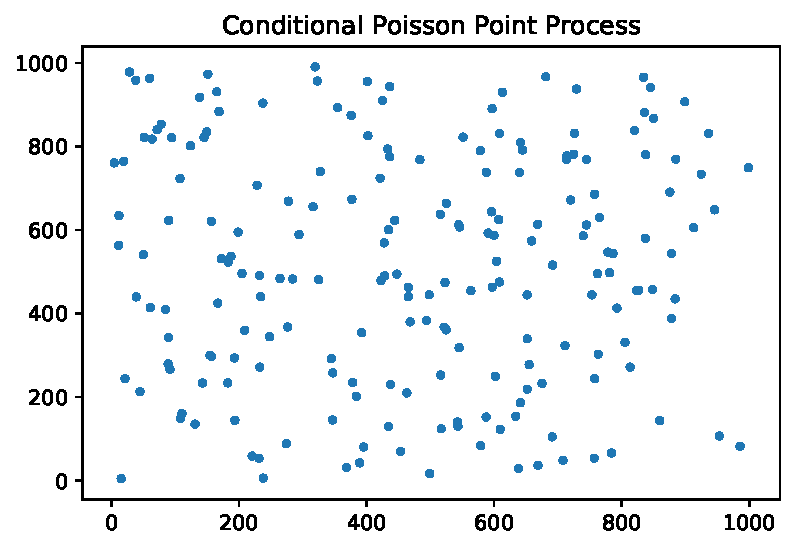
\includegraphics[width=.5\textwidth]{ppp.pdf}%
 \label{fig:point_process_generation:python:ppp}%
\end{figure}

\vspace*{-8pt}

\begin{python}
def cond_Poisson(nb_points, xmin, xmax, ymin, ymax):
    # Conditional Poisson Point Process
    # uniform distribution
    # nb_points: number of points
    # xmin, xmax, ymin, ymax: defined the domain (window)
    x = xmin + (xmax-xmin)*np.random.rand(nb_points)
    y = ymin + (ymax-ymin)*np.random.rand(nb_points);
    return x,y

def test_ppp():
    # testing function
    x,y = cond_Poisson(100, 0, 100, 0, 100);
    plt.plot(x,y,'+');
\end{python}

\subsection{Normal distribution}
The normal distribution is illustrated in Fig.\ref{fig:point_process_generation:python:npp}. Each marginal distribution (distribution on each axis) follows the normal distribution.

\begin{python}
def normal_distribution(nb_points, mu, sigma):
    # Normal distribution centered around the point mu with stdev sigma
    x = mu[0] + sigma[0]*np.random.randn(nb_points);
    y = mu[1] + sigma[1]*np.random.randn(nb_points);
    return x,y;
\end{python}

\begin{figure}[H]
 \centering\caption{Normal distribution of points around $(0,0)$, with $\sigma=(10, 20)$.}%
 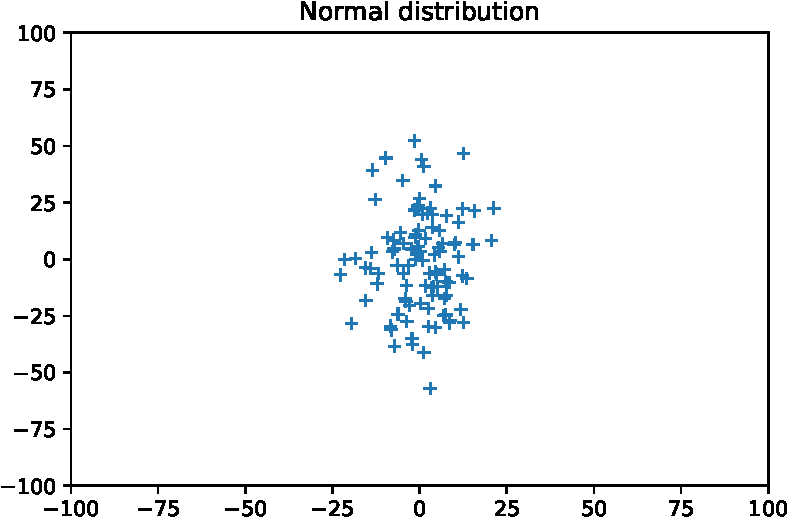
\includegraphics[width=.5\textwidth]{npp-crop.pdf}%
 \label{fig:point_process_generation:python:npp}%
\end{figure}

\vspace*{-10pt}


\subsection{Neyman-Scott Process}
Neymann-Scott point process is an agregated Poisson point process. It is illustrated in Fig.\ref{fig:point_process_generation:python:nspp}. It consists on a ``sub'' point processes generated at locations corresponding to a point process.

\begin{python}
def neyman_scott(nRoot, xmin, xmax, ymin, ymax, lambdaS, rSon):
    # Neyman-scott process simulation
    # nRoot: number of agregates
    # xmin, xmax, ymin, ymax: domain
    # lambdaS: number of points. lambda is a density, S is the spatial domain
    # rSon: radius around agregate (points are distributed in a square)
    
    # number of sons
    nSons = poisson.rvs(lambdaS, size=nRoot);
    # results    
    x=[];
    y=[];
    # father points coordinates
    xf,yf = cond_Poisson(nRoot, xmin, xmax, ymin, ymax);
    for i in range(nRoot):
        # loop over all agregates
        xs,ys = cond_Poisson(nSons[i], xf[i]-rSon, xf[i]+rSon, yf[i]-rSon, yf[i]+rSon);
        x = np.concatenate((x,xs), axis=0);
        y = np.concatenate((y,ys), axis=0);
    
    return x,y
\end{python}

\begin{figure}[H]
 \centering\caption{Neyman-Scott point process, with \pinline{lambdaS=10} and \pinline{rSon=10}.}%
 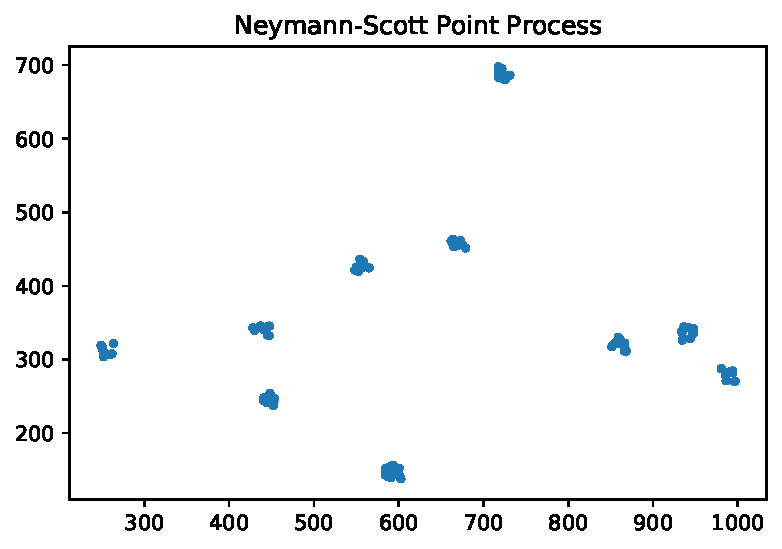
\includegraphics[width=.5\textwidth]{nspp.pdf}%
 \label{fig:point_process_generation:python:nspp}%
\end{figure}


\subsection{Gibbs Point Process}
Gibbs point process allows attraction and repulsion at different distances. It is illustrated in Fig.\ref{fig:point_process_generation:python:gpp}. The attraction/repulsion law is given by the following code for regular or agregated point process.

\begin{python}    
def exampleEnergyFunction(distance):
    """ This function returns e with the same size as distance
    e takes the value given in the variable energy according to the steps
    """
    e = np.zeros(distance.shape);
    e [distance <10] = 10;
    return e;

def agregatedEnergyFunction(distance):
    """ 
    Agregated energy function
    """
    e = np.zeros(distance.shape);
    e [distance <2] = 50;
    e [np.logical_and(distance>=2, distance<5)] = -10;
    e [np.logical_and(distance>=5, distance<10)] = 5;

    return e;
\end{python}

The evaluation of the energy computes all pairwise distances and sum up the energies associated, or it computes the distances between one single point to a set of points.

\begin{python}
def energy(P, eFunction=exampleEnergyFunction):
    """
    This computes the energy in the set of points P, with the energy function
    given as a parameter.
    return a float value
    """
    P = np.transpose(P);
    d = pdist(P);
    e = exampleEnergyFunction(d);
    return np.sum(e);
    
def energyFromPoint(p, P, eFunction=exampleEnergyFunction):
    """
    Compute energy from point p to all points of P
    """
    dist = np.sqrt((p[0] - P[0,:])**2 + (p[1] - P[1,:])**2);
    ee = eFunction(dist);
    return np.sum(ee);
\end{python}

The principle of the algorithm is to iteratively add one point that minimizes the energy after several trials. In order to speed up the process, notice that only one point is moved, and it is thus sufficient to only compute the distances from this point to all others.
\begin{python}
def gibbs(nb_points, xmin, xmax, ymin, ymax, nbiter, eFunction=exampleEnergyFunction):
    """
    Gibbs point process
    xmin, xmax, ymin, ymax represents the spatial window
    nb_points: number of generated points
    nbiter: number of iterations
    returns (x,y) coordinates of the points
    """
    
    # start with a Poisson Point Process
    x,y = spat_pp.cond_Poisson(nb_points, xmin, xmax, ymin, ymax);
    nb_moves = 0;
    e_prev = energy(np.vstack((x,y)), eFunction);
    print("initial energy: {0:f}".format(e_prev));

    for i in range(nbiter):
        # choose a random point
        j = np.random.randint(0, nb_points);
        x2 = np.delete(x, j);
        y2 = np.delete(y, j);
        
        P = np.vstack((x2, y2));
        e1 = energyFromPoint([x[j], y[j]], P, eFunction);
        
        for m in range(10):
            xm,ym = spat_pp.cond_Poisson(1, xmin, xmax, ymin, ymax);
            
            e2 = energyFromPoint([xm, ym], P, eFunction);
            if e2<e1:
                nb_moves+=1;
                x[j]=xm;
                y[j]=ym;
                e1=e2;
          
    print( "Number of moves: " + str(nb_moves));
    print("Final energy:    " + str(e1));
    return x, y
\end{python}

\begin{figure}[H]
 \centering\caption{Gibbs point processes (with the same number of points).}%
 \subfloat[Regular Gibbs point process.]{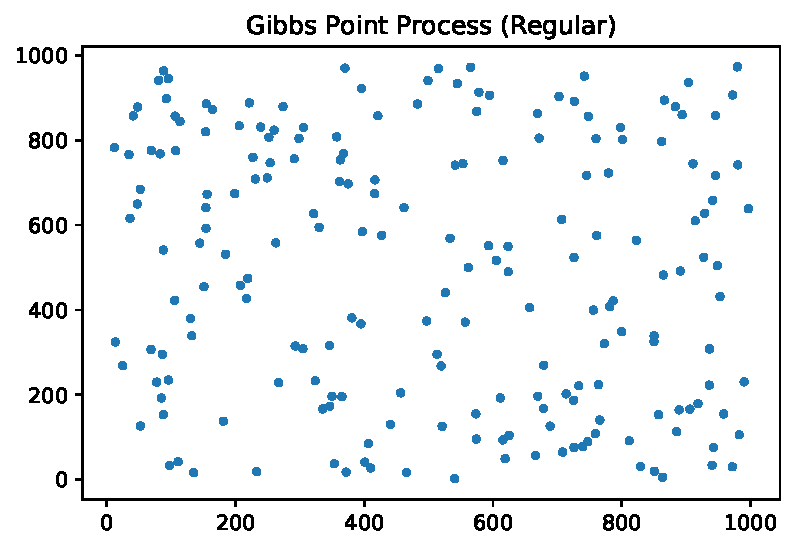
\includegraphics[width=.45\textwidth]{gpp.pdf}}\hfill
 \subfloat[Agregated Gibbs point process.]{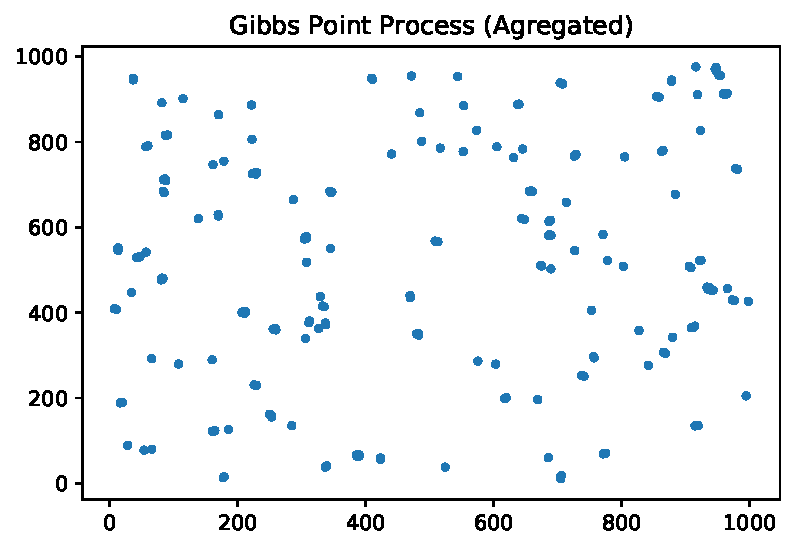
\includegraphics[width=.45\textwidth]{gpp_a.pdf}}%
 \label{fig:point_process_generation:python:gpp}%
\end{figure}

\subsection{Ripley functions}
The Ripley functions are useful to characterize a point process. Agregation and repulsion can be observed with regard to the distance (see Fig.\ref{fig:point_process_generation:python:ripley}). Notice that this function is biased because points in border of window are counted as points in the center. This could be corrected by the use of \pinline{scipy.spatial.distance.cdist}.

\begin{python}
def ripley(x, y, xmin, xmax, ymin, ymax, edges):
    # Ripley K and L functions, vals is values of radius
    # this function has border effects!
    # x, y: coordinates of points
    # xmin, xmax, ymin, ymax: window
    # edges: values of bins for histogram evaluation
    
    # number of points    
    nb_points = x.size;
    
    # compute pairwise distances
    P = np.transpose(np.vstack((x,y)));
    d =  pdist(P);
    
    # compute cumulative histogram
    h,edges = np.histogram(d, edges);
    H = np.cumsum(h);
    
    # normalization of K    
    K = 2*H/nb_points;
    area = (xmax-xmin) * (ymax-ymin);
    density = float(nb_points) / area;
    K = K / density;
    
    # L
    L = np.sqrt(K/np.pi);
    
    # edge values
    vals = edges[:-1] + np.diff(edges);
    
    return K, L, vals
\end{python}

\begin{figure}[H]
 \centering\caption{Ripley functions.}%
 \subfloat[Ripley K function.]{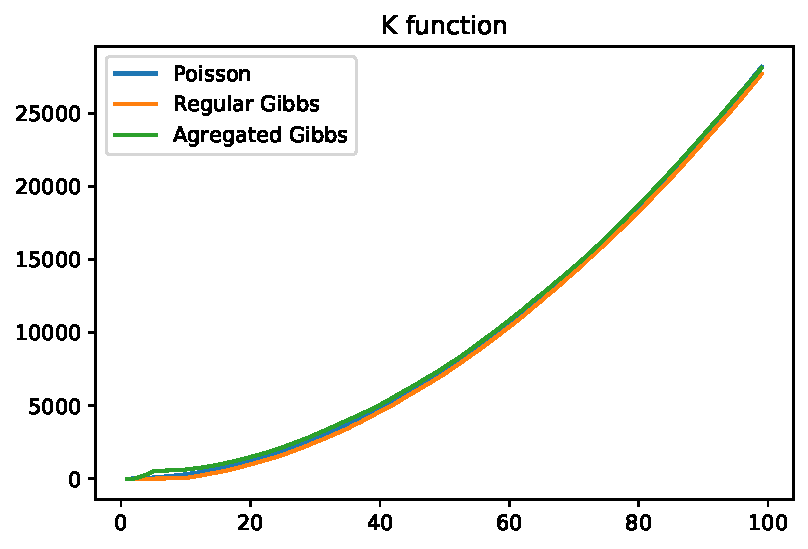
\includegraphics[width=.45\linewidth]{ripley_python.pdf}}
 \hfill
 \subfloat[Ripley L function.]{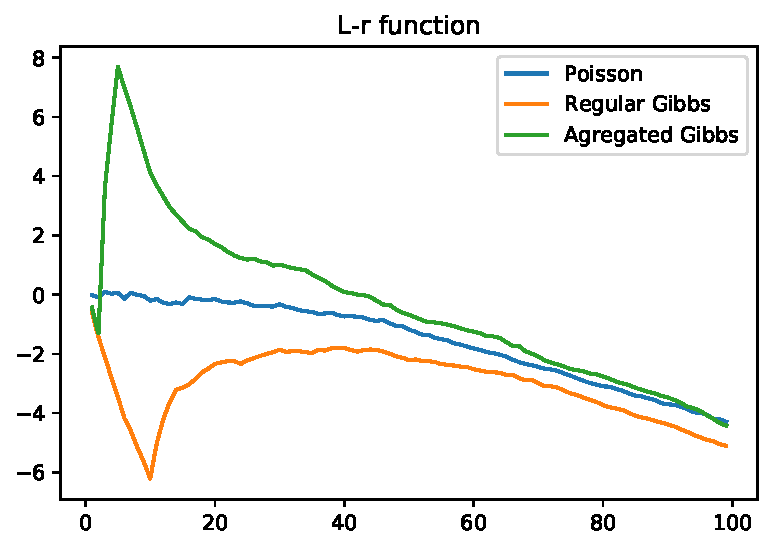
\includegraphics[width=.45\textwidth]{ripley_L_python.pdf}}%
 \label{fig:point_process_generation:python:ripley}%
\end{figure} 

\subsection{Marked Point Process}
An illustration is presented in Fig.\ref{fig:point_process_generation:python:marked}. The algorithm simply consists in adding two new random variables in order to generate the radius and the color of each point.

\begin{python}
def marked(nb_points, xmin, xmax, ymin, ymax):
    """
    marked point process
    """
    
    # points
    x,y = spat_pp.cond_Poisson(nb_points, xmin, xmax, ymin, ymax);
    
    # first mark: radii
    sigma = 5;
    mu = 10;
    r = sigma * np.random.randn(nb_points) + mu;
    r[r<0.1] = 0.1;
    
    # second mark: colors
    nb_colors = 10;
    c = np.random.randint(nb_colors,size = nb_points);
    
    # plot
    plt.scatter(x, y, r**2, c, alpha=.5);
	 
	 # save pdf figure
	 plt.savefig("marked.pdf");
    
nb_points = 100;
N=100;
marked(nb_points, 0, N, 0, N);
\end{python}

\begin{figure}[H]
 \centering\caption{Marked point process.}%
 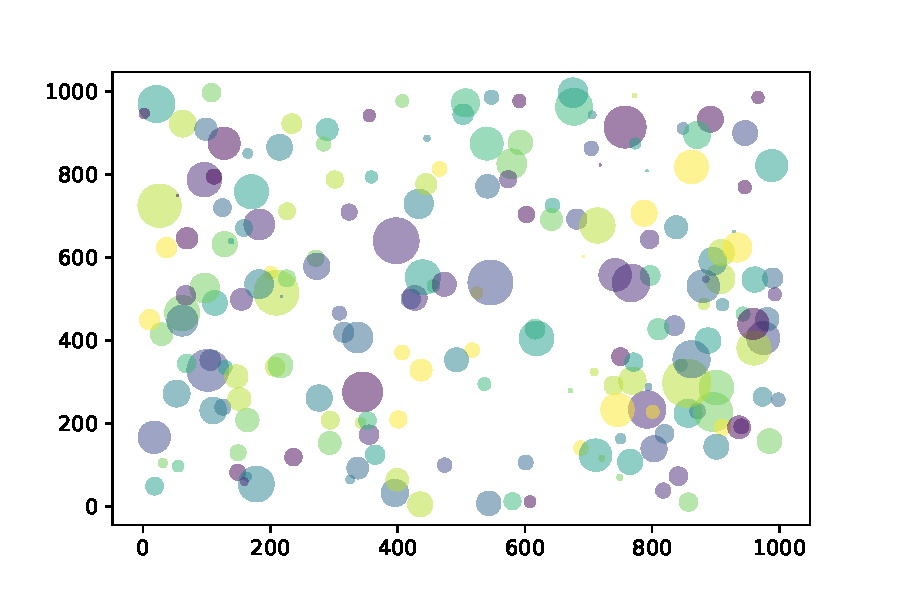
\includegraphics[width=.8\linewidth]{marked.pdf}%
 \label{fig:point_process_generation:python:marked}%
\end{figure}
